\chapter{Introduction}\label{ch:introduction}

%======================================================================

\section{Motivation}\label{sec:motivation}

Since Roentgen’s discovery of X-rays in 1895, medical imaging has
advanced significantly, with modalities like radionuclide imaging,
ultrasound, \gls{CT}, \gls{MRI}, and digital radiography emerging over the past
50 years. Modern imaging extends beyond image production to include
processing, display, storage, transmission and analysis.
\cite{Zhou2021}.
Other \gls{MITs} have arose during the last decades, some of them
implying only the examination of certain pieces or tissues
instead of complete patients, like histopathological images, which
are images of tissue samples obtained from biopsies or surgical
resections and are widely used for the diagnosis of diseases like
cancer through \gls{WSI} scanners \cite{Rashmi2021}.

Along with the advances in technologies for medical images acquisition,
computational technologies on pattern recognition and artificial intelligence
have also emerged, allowing the development of \gls{CAD} systems based on
machine learning algorithms. These systems aim to assist physicians
in the diagnosis and treatment of diseases, by providing a second
opinion or by automating the analysis of medical images.
\cite{Panayides2020}. One of the most used tasks in which machine
learning technologies is being used in the universe of medical images
is \gls{ISS}, which consists of assigning a label to each pixel in an image
according to the object it belongs to. This task is crucial for the development
of \gls{CAD} systems, as it allows the identification of \gls{ROI} in
the images, which can be used to detect and classify diseases
\cite{Azad2024}.

The application of Machine Learning in medical imaging has grown
significantly, with key tasks including classification, segmentation,
anomaly detection, super-resolution, image registration, and
synthetic image generation \cite{BritoPacheco2025}. Among imaging
modalities, X-rays and \gls{CT} scans are widely used for classification
and anomaly detection, especially in pulmonary and oncological
applications. \gls{MRI} and ultrasound play a crucial role in segmentation
and resolution enhancement, while PET/SPECT imaging is essential for
anomaly detection in oncology and neurodegenerative diseases
\cite{BritoPacheco2025}.
Histopathology is rapidly gaining prominence, particularly in segmentation and
feature extraction, where AI-driven techniques aid in automated
cancer diagnosis and tissue structure analysis. The integration of
Deep Learning in histological image processing is revolutionizing
pathology, enabling more precise and efficient diagnostics. A brief
comparison of the tasks and medical image types
based on recent literature review, can be seen in Figure
\ref{fig:medical_image_analysis}. \cite{YuEtAl2025},
\cite{BritoPacheco2025}, \cite{RyouEtAl2025},
\cite{DingyiEtAl2025}, \cite{BehnazEtAl2025}

\begin{figure}
  \centering
  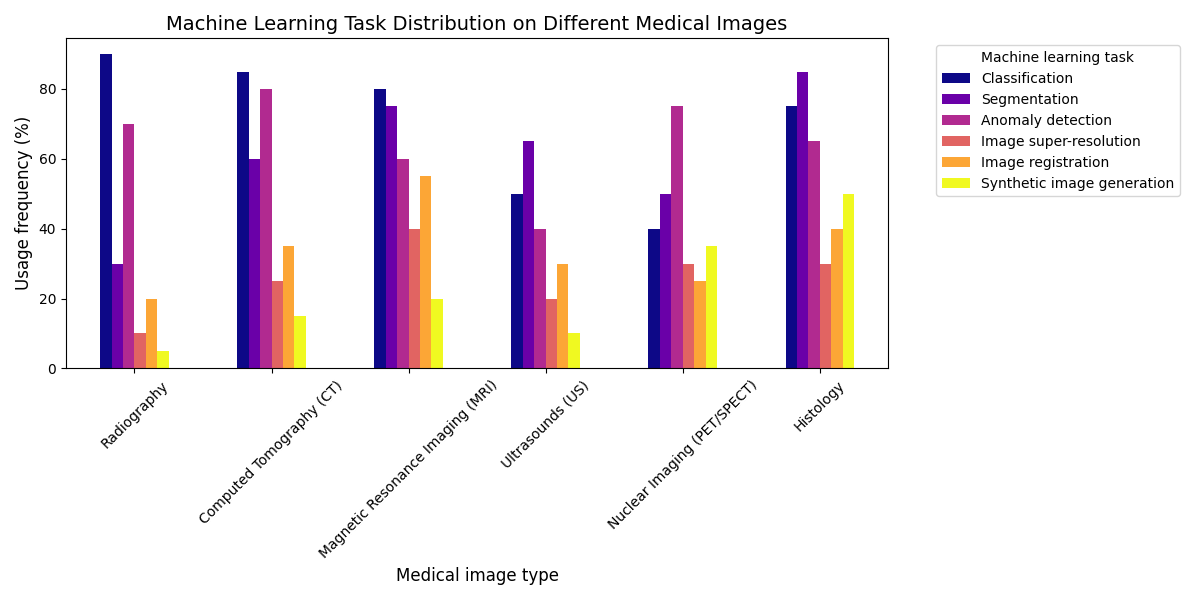
\includegraphics[width=0.9\textwidth]{Cap1/Figures/comparative-tasks-and-medical-image-types.png}
  \caption{Estimation of the popularity of tasks and medical image
    types based on
  recent literature review (count of referenced terms).}
  \label{fig:medical_image_analysis}
\end{figure}

For solving the different requirements of tasks in medical images, a
variety of computational techniques have been developed
\cite{Zhou2021}. Initially, these needs were covered with simple
morphological filters, which implied no training process or
elaborated optimization. However, as the complexity of the tasks
increased, the need for more sophisticated techniques arose, leading
to the application of advanced statistical tools and machine learning
algorithms like Support Vector Machines, Decision Trees, and SGD
Neural Networks \cite{Avanzo2024}. The coevolution of advances in medical image
acquisition, computational power (i.e. Moore's law) and
statistical/mathematical techniques have led to a convergence for
merging state of the art algorithms with medical imaging
\cite{Shalf2020}. Figure \ref{fig:medical-ai-timeline} shows a brief
timeline of coevolution between some conspicuous advances in
computational pattern recognition and its medical applications in
different scopes (besides medical imaging) \cite{Avanzo2024}.

\begin{figure}
  \centering
  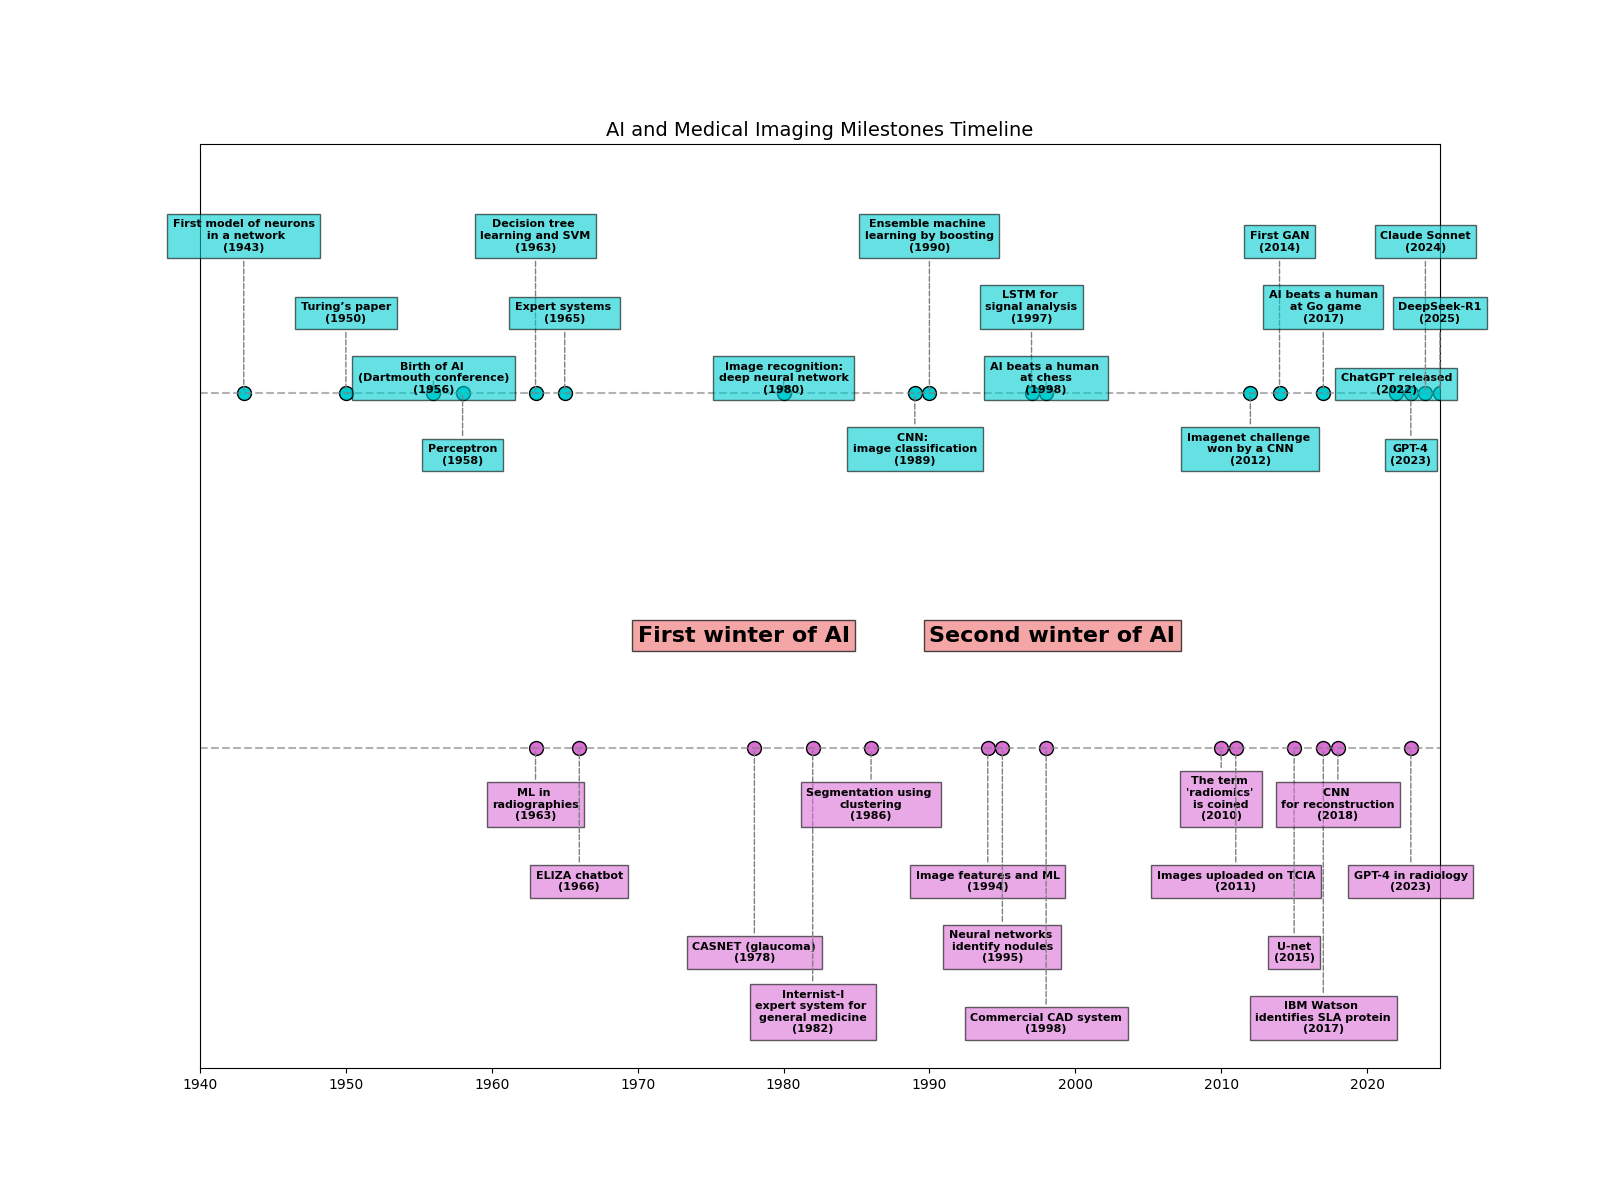
\includegraphics[trim={5cm 2cm 5cm
  0},width=0.9\textwidth]{Cap1/Figures/medical-ai-timeline.png}
  \caption{AI and machine learning in medical imaging brief timeline.}
  \label{fig:medical-ai-timeline}
\end{figure}

\gls{CNN} have been widely used in \gls{SS} tasks, as they have outperformed
traditional machine learning algorithms in this task for both medical
and non medical images \cite{XuYan2024} \cite{Sarvamangala2022}.
However, most \gls{CNN} architectures are deep, which imply
a necessity of a large amount of data to train them. This introduces
a problem since both the acquisition and annotation of medical images
are expensive and time-consuming processes. This is especially true
for \gls{ISS} tasks, as they require pixel-level annotations, which
is taxing in terms of cost, time and logistics involved
\cite{Bhalgat2018}. Other fashions face this problem through less expensive
annotation strategies like bounding boxes or anatomical landmarks for
being used in a semi-supervised strategy \cite{Shah2018}.

%% CHECKED

Many medical images datasets however, contain a high variability in
class sizes and variations in colors, which is specially noticeable
in histopathological images because of the usage of different
staining and other factors which can affect the color of the images
(see section \ref{sec:staining-techniques}).
This variability can lead to a significant loss of efficiency of
machine learning models when using a mixed supervision strategy, as
the model can be biased towards the most common classes or colors in
the dataset \cite{Shah2018}.

This is were other solutions arise to tackle the problem of the weak
image annotation while maintaining low costs. One of these solutions
is crowdsourcing strategy, which consists of having multiple annotators
labeling the same image, and then combining the labels to obtain a
consensus label \cite{LuEtAl2023}. This strategy can lead to a
labeling cost reduction when different levels of expertise are
combined, since the crowd may be composed of both experts and laymen,
being the latter less expensive to hire \cite{Lopez2023}.

Recently, diagnosis, prognosis and treatment of cancer have heavily
relied on histopathology, where tissue samples are obtained through biopsies or
surgical resections and critical information that helps
pathologists determine the presence and severity of malignancies
\cite{LopezEtAl2024}. The segmentation of histopathological images
enables precise identification of structures such as nuclei, glands, and tumors,
which are essential for assessing disease progression and treatment
response \cite{Rashmi2021}. Accurate segmentation is particularly
crucial in digital pathology, where whole-slide images (\gls{WSI})
are analyzed using AI-powered \gls{CAD} systems to support
clinical decision-making \cite{LopezEtAl2024}.

A major challenge in histopathological image segmentation arises from
the variability in annotations provided by different pathologists.
Unlike natural images, where object boundaries are often
well-defined, histological structures may have ambiguous borders,
leading to inconsistencies among annotators \cite{Lopez2023}. Because of this,
crowdsourcing labeling is one of the most popular approaches, as
illustrated in Figure \ref{fig:multiannotator_segmentation},
an example of how histopathological images are segmented by
multiple experts, showing some variations in label assignment
\footnote{obtained from a real world Triple Negative Breast
Cancer (TNBC) dataset published in \cite{Lopez2023}}. These
discrepancies highlight the need for models that can handle
annotation uncertainty effectively. Leveraging crowdsourcing
strategies and machine learning techniques that infer annotator
reliability can enhance segmentation performance while reducing costs.
\begin{figure}
  \centering
  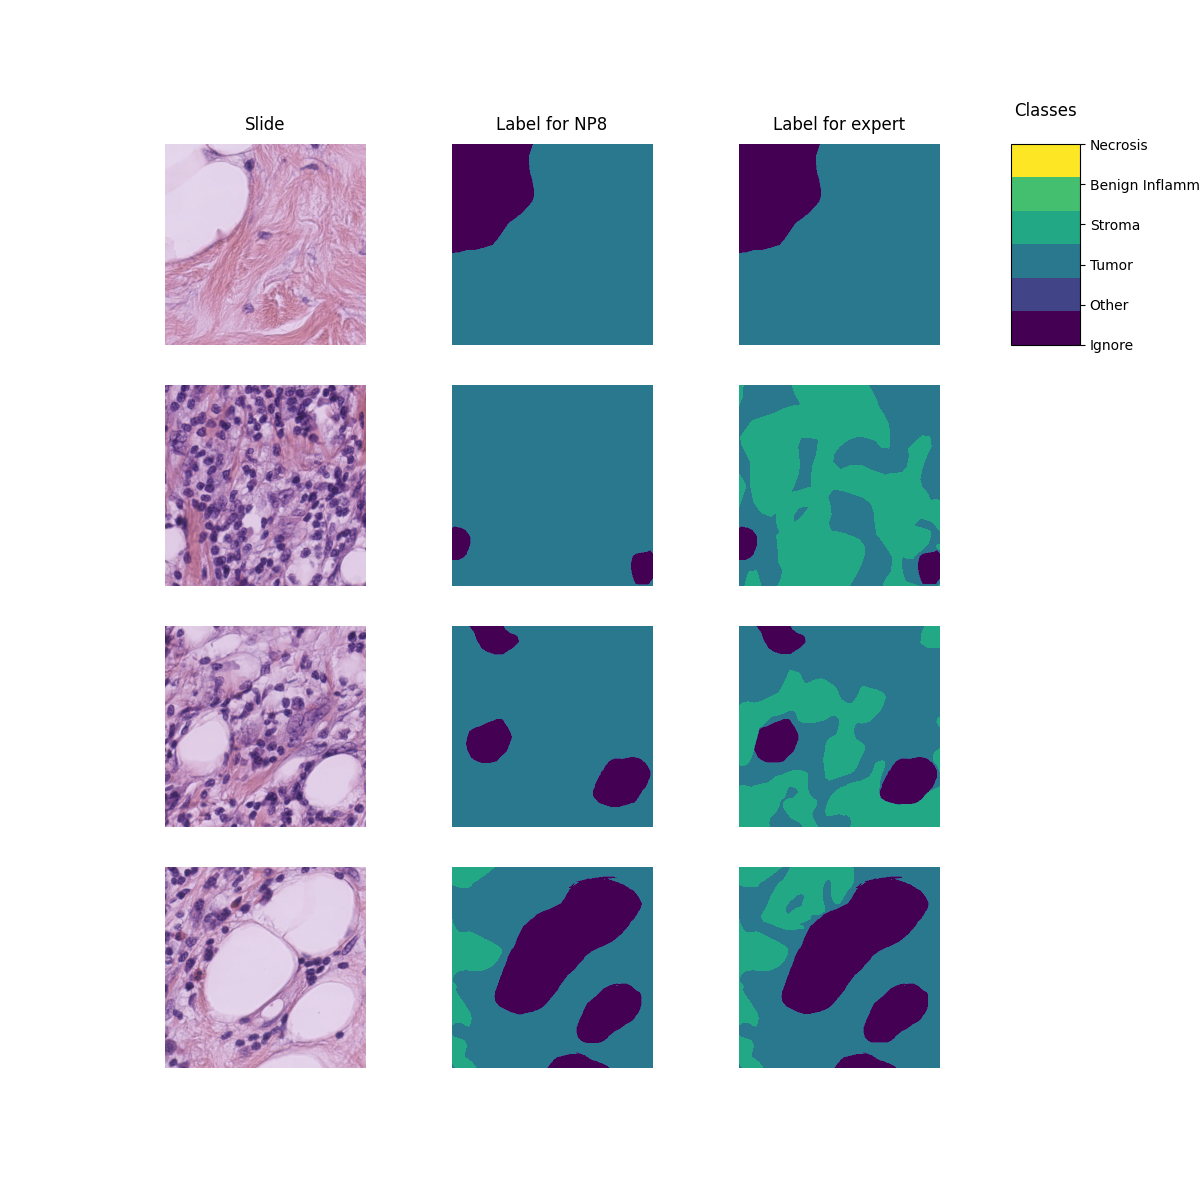
\includegraphics[width=0.9\textwidth]{Cap1/Figures/multiannotator-segmentation.png}
  \caption{Example of a histopathological image segmented by multiple
  annotators, illustrating variations in label assignment.}
  \label{fig:multiannotator_segmentation}
\end{figure}
\section{Problem Statement}\label{sec:state_of_art}

% ==============================
% Problem Statement Chapter
% ==============================

% Highlight the issue of inter-observer variability and the need for
% robust models that can learn from inconsistent labels.

Throughout the development of medical technology and \gls{CAD}, the
task of \gls{ISS} has become a crucial step in delivering precise diagnosis
and treatment planning \cite{Giri_Bhatia_2024}. Particularly, in the
area of histopathological studies, the usage of Whole Slide Images
(\gls{WSI}) is rather common since this method delivers high quality
imaging and allows for the diagnosis of diseases like cancer
\cite{YujiaEtAl2024}.

\gls{ISS} task consists of assigning a label to each pixel
in an image according to the object it belongs to. Accurate
segmentation is essential for the development of \gls{CAD} systems,
as it allows the identification of regions of interest (\gls{ROI}) in
the images, which can be used to detect and classify diseases and
hence, treatment planning \cite{Sarvamangala2022}. However, modern computational
solutions for \gls{ISS} tasks involve the use of deep learning, which
mostly rely large amounts of labeled data to train the models
on supervised learning techniques. This means that the model is trained on
a dataset with ground-truth labels, which are assumed to be correct
and consistent across all samples. In practice, this assumption is
often violated due to the high technical complexity of labeling these
segments \footnote{compared to a more trivial task like image classification
on ordinary an well known classes like MNIST}.

% The Multiple-Labelers Challenge
% Detail how medical images often require annotations from multiple
% experts with varying levels of expertise.
% Discuss common issues such as random errors (accidental mistakes)
% and expertise errors (systematic biases due to limited knowledge).
% Reference existing approaches that either require ground-truth
% labels or additional supervision to model labeler performance explicitly.

The process of labeling medical images is often managed with the help of
specialized software tools that allow the annotators to draw the
regions, delivering an standard format for the labeled
masks \cite{Habis2024}.
Despite the help of these tools, the labeling process in \gls{WSI} can have high
costs, as it requires long hours of work from specialized personnel.
Because of cost constraints in many medical institutions, the labeling processes
is often done by multiple labelers with varying levels of expertise, equalizing
the cost of the labeling process. However, this strategy can lead to
inconsistent labels, as the consensus between the labelers may not be
exact due to the diversity in depth of knowledge and experience of
the labelers \cite{XuYan2024}.
These inconsistencies are mostly represented in the subsections
\ref{subsec:expertise_levels} and \ref{subsec:technical_constraints}.

\subsection{Variability in Expertise Levels}\label{subsec:expertise_levels}

One of the primary sources of inter-observer variability in medical
image segmentation is the difference in expertise levels among
annotators \cite{Lopez2023}. Experienced radiologists and
pathologists tend to produce highly precise annotations, whereas
novice labelers may introduce systematic biases due to their limited
familiarity with subtle image features. Studies have demonstrated
that annotation accuracy \textit{tends} to improve with experience, yet medical
institutions often rely on a mix of annotators to manage costs and
workload distribution \cite{LuEtAl2023}.

The training background of annotators and institutional guidelines
play a crucial role in shaping labeling practices. Different medical
schools and hospitals may adopt distinct segmentation protocols,
leading to inconsistencies when datasets are combined from multiple
sources \cite{Lopez2023}. For example, some institutions may emphasize
conservative delineation of tumor boundaries, while others adopt a
more inclusive approach. Such variations contribute to systematic
biases in medical image datasets \cite{BanerjeeEtAl2025}.

Medical images frequently contain structures with ambiguous
boundaries, making segmentation inherently subjective. For instance,
tumor margins in histopathological slides may not have well-defined
edges, leading to variations in how different annotators delineate
the regions of interest \cite{Carmo2025}. These discrepancies arise not only
from technical expertise but also from differences in perception and
interpretation.

\subsection{Technical Constraints and Image
Quality}\label{subsec:technical_constraints}

Technical constraints in medical imaging, such as resolution
differences, noise levels, and contrast variations, can significantly
impact segmentation accuracy. Lower-resolution images may obscure
fine structures, leading to inconsistencies in boundary delineation
\cite{ZhouEtAl2024}.

When combined with long sessions, bad images might
also increase the cognitive load of the annotators, leading to
fatigue and reduced precision in labeling \cite{KimYujinAndLee2024}.
This is particularly relevant in histopathological studies, where the
staining process and tissue preparation can introduce color
variations and artifacts that affect image quality, even if the same scanning
equipment is used \cite{Karthikeyan2023}.

\begin{figure}
  \centering
  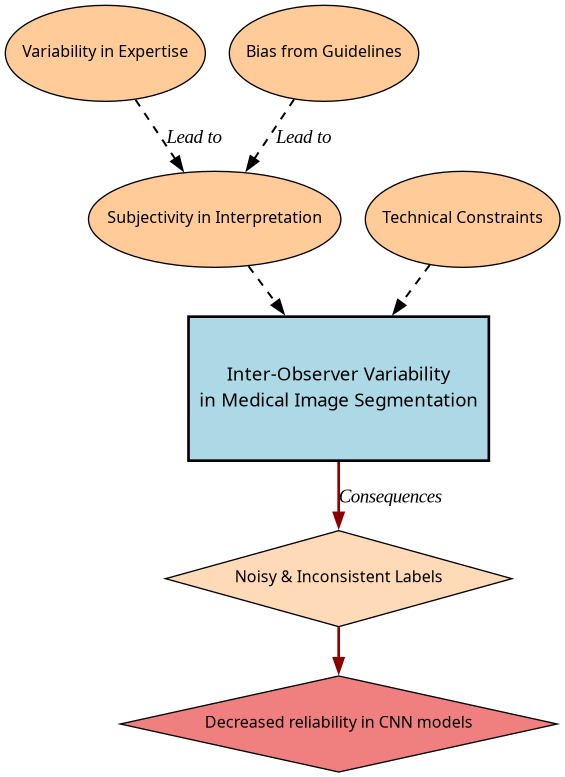
\includegraphics[width=0.7\textwidth]{Cap1/Figures/problem_statement_diagram.png}
  \caption{Summary diagram for problem Statement}
  \label{fig:problem_statement_diagram}
\end{figure}

\subsection{Research Question}

Given the challenges posed by inconsistent labels in medical image
segmentation, this work aims to address the following research
question:

\researchquestion{How can we develop a learning approach for
  \gls{ISS} tasks in medical images that can adapt to inconsistent
  labels without requiring explicit supervision of labeler
  performance, while addressing challenges related to variability in
  expertise levels and technical constraints, and maintaining
interpretability, generalization, and computational efficiency?}
\section{Literature review}\label{sec:state_of_art}

Certainly, in general \gls{ML} classification tasks \footnote{In this
  work, image segmentation is considered as a particular case of classification
in which target classes are assigned pixel-wise.} where multiple
annotators are involved, \gls{MV} is by far the simplest
possible approach to implement. This concept was born multiple times
and divergently in multiple fields, but it was described as relevant
for \gls{ML} and pattern recognition labeling for classification in
\cite{LamAndSuen1997}, in which the approach is exposed as simple,
yet powerful. The authors describe the \gls{MV} as a method that can
be used to improve the accuracy of classification tasks by combining
the labels of multiple annotators. The method is based on the
assumption that the majority vote of the annotators is more likely to
be correct than the vote of a single annotator. The authors also
describe the method as a straightforward way to improve the accuracy
of classification tasks without the need for complex algorithms or
additional data. The authors also prove this method to deliver very
similar results to more complicated approaches (Bayesian, logistic
regression, fuzzy integral, and neural network) in the
particular task of \gls{OCR}. Despite its simplicity, modern
solutions for delivering accurate medical image segmentation models
still rely on Majority Voting at some stage, like \cite{Elnakib2020},
which uses a majority voting strategy for delivering a final output
based on the labels of multiple models (VGG16-Segnet, Resnet-18 and
Alexnet) in \gls{CT} images for Liver Tumor Segmentation, or
\cite{Lopez2023}, which uses \gls{MV} for combining noisy annotations
as an additional annotator to be included in the deep learning solution.
Majority voting as a technique for setting a pseudo ground truth label
is a powerful approach for its simplicity in many use cases in which
the target to be labeled is not tied to an expertise related task,
otherwise, the assumption of equal expertise among the labelers can
be a source of bias in the final label, which is not desirable in the
case of highly technical annotations like medical images.
In subsection \ref{subsec:expertise_levels_lit_review}, we will be
reviewing literature which no longer assumes the naive approach of
equal expertise among labelers and face the challenge of learning
from inconsistent labels.

\subsection{Facing annotation variability in medical
images}\label{subsec:expertise_levels_lit_review}

Learning from crowds approaches in general face the challenge of
not having a ground truth label and hence, an intrinsic difficulty in
measuring the real reliability of the labelers annotations. Some
approaches assume beforehand a certain level of expertise for each
labeler based on experience as an input, like in
\cite{TianEtZhu2015}, which introduce the concept of max margin
majority voting, using the reliability vector as weights for the
weights for the binary and multiclass classifier. The crowdsourcing
margin is the minimal difference between the aggregated score of the
potential true label and the scores for other alternative labels.
Accordingly, the annotators' reliability is estimated as generating
the largest margin between the potential true labels and other
alternatives. The problem introduced in this approach is assuming an
stationary reliability per expert across the whole input space, which
is imprecise since annotators performance may change between
different tasks or even between different regions of the same image.

% REVIEW
\subsubsection{STAPLE Mechanism}

The \gls{STAPLE} algorithm, introduced in \cite{WarfieldEtAl2004}
is a probabilistic framework that estimates a hidden true
segmentation from multiple segmentations provided by
different raters. It also estimates the reliability of each rater by
computing their sensitivity and specificity.

The \gls{STAPLE} algorithm's goal is to maximize the log likelihood function:

\begin{equation}\label{eq:staple_likelilhood}
  (\mathbf{\hat{p}}, \mathbf{\hat{q}}) = \arg\max_{\mathbf{p}, \mathbf{q}} \ln
  f(\mathbf{D},
  \mathbf{T} \mid \mathbf{p}, \mathbf{q}).
\end{equation}

Where $\mathbf{D}$ is the set of segmentations provided by the raters,
$\mathbf{T}$ is the hidden true segmentation, $p$ is the sensitivity
and $q$ is the specificity of the raters.

This is achieved by using the Expectation-Maximization algorithm to
maximize the log likelihood function in equation, which is done iteratively
with step computations:

\begin{equation}
  \begin{split}
    (p_j^{(k)}, q_j^{(k)}) = \arg\max_{p_j, q_j} \sum_{i:D_{ij}=1}
    W_i^{(k-1)} \ln p_j \\
    &+ \sum_{i:D_{ij}=1} \left(1 - W_i^{(k-1)}\right) \ln (1 - q_j) \\
    &+ \sum_{i:D_{ij}=0} W_i^{(k-1)} \ln (1 - p_j) \\
    &+ \sum_{i:D_{ij}=0} \left(1 - W_i^{(k-1)}\right) \ln q_j.
  \end{split}
\end{equation}

The capacity of STAPLE to accurately estimate the true segmentation,
even in the presence of a majority of raters generating correlated
errors, was demonstrated, which makes it theoretically a strong
choice for setting a ground-truth in binary or multiclass medical
\gls{ISS} tasks.

The popularity and performance of \gls{STAPLE} has led to its
usage in modern applications medical image, 3d spatial images due to
its assumption of decision space being based on voxel-wise decisions,
like the authors in \cite{GrefveEtAl2024} which applied the algorithm
on \gls{PET} images. Other authors still rely heavily on STAPLE for
setting a ground truth consensus for histopathological images, like
\cite{QiuEtAl2022}.

However, the \gls{STAPLE} algorithm has some limitations. It
assumes independent rater errors, which may not hold in practice,
leading to biased estimates. STAPLE is also sensitive to low-quality
annotations, potentially degrading final segmentations if the weights
are not initialized correctly. The algorithm tends to over-smooth
results, blurring fine details, and struggles with multi-class
segmentation. Computationally, it is expensive due to its iterative
EM approach. Additionally, STAPLE cannot correct systematic biases in
annotations and depends on initial estimates, impacting accuracy.
Lastly, the estimated performance levels lack interpretability,
making it difficult to assess annotator reliability effectively.

Finally, this work contemplates \gls{STAPLE} as useful for ground
truth estimation given the existence of multiple labelers for an
input \gls{WSI}, but not that useful for providing annotations of structures on
new and unlabeled images, hence being a good support for other methods.

\subsubsection{Chained Gaussian Processes}

Other works like \cite{GilGonzalesEtAl2025} proposed a novel approach

\subsection{Strategies for handling low-quality images}

The problem of low-quality images and noisy annotations has been
tackled with various strategies. One such approach is the use of deep
learning models that incorporate loss functions designed to mitigate
the effects of unreliable labels. Traditional methods such as
Majority Voting (MV) or Expectation-Maximization (EM) have been
widely used for aggregating multiple annotators' inputs. However,
they assume a homogeneous reliability of annotators, which may not
hold in real-world scenarios.

A more recent approach was proposed by \cite{TrianaEtAl2023},
introducing a Generalized Cross-Entropy-based Chained Deep Learning
(GCECDL) framework. This method addresses the limitations of
traditional label aggregation techniques by modeling each annotator's
reliability as a function of the input data. The approach effectively
mitigates the impact of noisy labels by using a noise-robust loss
function, balancing Mean Absolute Error (MAE) and Categorical
Cross-Entropy (CE). Unlike prior approaches, GCECDL accounts for the
dependencies among annotators while encoding their non-stationary
behavior across different image regions. Their experiments on
multiple datasets demonstrated superior predictive performance
compared to state-of-the-art methods, particularly in cases where
annotations were highly inconsistent.

This strategy is especially relevant for handling low-quality medical
images, where expert annotations may be inconsistent, and traditional
consensus-based approaches fail to account for varying expertise
levels. By leveraging deep learning with robust noise-handling loss
functions, the reliability of segmentation models can be significantly improved.


\section{Aims}\label{sec:objectives}

With the mentioned considerations in section \ref{sec:state_of_art}
in mind, this work proposes a novel approach for \gls{ISS} tasks in
medical images, which aims to train a model whose learning approach
is adaptive to the labeler performance. This is done by introducing a
loss function capable of inferring the best possible segmentation
without needing separate inputs about the labeler performance. This
loss function is designed to implicitly weigh the labelers based on
their performance, with the presence of an intermediate reliability
map allowing the model to learn from the most reliable labelers and
ignore the noisy labels. This approach differs from existing
\gls{CNN}-based segmentation models, as it does not require explicit
supervision of the labeler performance, making it more generalizable
and adaptable to different datasets and labelers.
\subsection{General Aim}

The main purpose of this work is to develop a novel approach for
\gls{ISS} tasks in medical images, which can adaptively infer the best
possible segmentation without needing separate inputs about the
labeler performance. This approach is expected to outperform the
segmentation performance of other state of the art approaches,
eliminate the need for explicit labeler supervision, and enhance
automation in medical image analysis.

%----------------------------------------------------------------------
\subsection{Specific Aims}

\begin{itemize}

  \item To develop a novel loss function for \gls{ISS} tasks in
    medical images, capable of inferring the best possible
    segmentation without needing separate inputs about the labeler
    performance.

  \item Introducing a tensor map which codifies the reliability of
    each labeler, allowing the model to implicitly weigh the labelers
    based on their performance across the mask and classes space.

  \item To develop and test a deep learning model for \gls{ISS} tasks
    in medical images, which can learn from inconsistent labels and
    improve the segmentation performance compared to other solutions
    in state of the art.

\end{itemize}


\clearpage
\section{Outline and Contributions}

As an output of this work, some contributions were made to the field of
\gls{ISS} in medical images. The main contributions are:

\begin{itemize}
  \item A novel loss function for \gls{ISS} tasks in medical images capable of
    inferring the best possible segmentation and codifying the
    reliability of the labelers without needing separate inputs about
    the labeler performance or multiple networks to be trained.
  \item A Chained Deep Learning model for \gls{ISS} tasks in medical
    images, which can learn from inconsistent labels and improve the
    segmentation performance outperforming state of the art
    approaches on a Triple Negative Breast Cancer histopathology dataset.
  \item A mechanism for noisy annotations emulations by using networks
    encoding layers weight disturbance for building crowdsourced
    version of the well known Oxford-IIIT Pet Dataset.
  \item A python package for using the proposed loss function and
    architecture in \gls{CNN} models for \gls{ISS} tasks in medical images.
    \footnote{https://pypi.org/project/seg\_tgce/}
  \item Triple negative breast cancer and Oxford-IIIT Pet Datasets
    mapping as lazy loaders for the proposed loss function ready to go in
    the package.
    \footnote{https://seg-tgce.readthedocs.io/en/latest/experiments.html}
  \item A public Github repository with the code used in this work.
    \footnote{https://github.com/blotero/seg\_tgce}
\end{itemize}
